% This is samplepaper.tex, a sample chapter demonstrating the
% LLNCS macro package for Springer Computer Science proceedings;
% Version 2.20 of 2017/10/04
%
\documentclass[runningheads]{llncs}
%
\usepackage{graphicx}
% Used for displaying a sample figure. If possible, figure files should
% be included in EPS format.
%
% If you use the hyperref package, please uncomment the following line
% to display URLs in blue roman font according to Springer's eBook style:
% \renewcommand\UrlFont{\color{blue}\rmfamily}
\usepackage{amsmath}

\begin{document}
%
\title{Deep triplet network adopting the kernel and the range space learning for Wi-Fi signature verification}
%
%\titlerunning{Abbreviated paper title}
% If the paper title is too long for the running head, you can set
% an abbreviated paper title here
%
\author{YoungWoong KWON\inst{1} \and
Jooyoung Kim \inst{1} \and
Kar-Ann Toh\inst{1}}
%
\authorrunning{F. Author et al.}
% First names are abbreviated in the running head.
% If there are more than two authors, 'et al.' is used.
%
\institute{Yonsei University \and
\email{lncs@springer.com}\\
\url{http://www.springer.com/gp/computer-science/lncs} \and
ABC Institute, Rupert-Karls-University Heidelberg, Heidelberg, Germany\\
\email{\{abc,lncs\}@uni-heidelberg.de}}
%
\maketitle              % typeset the header of the contribution
%
\begin{abstract}
The abstract should briefly summarize the contents of the paper in
15--250 words.

\keywords{First keyword  \and Second keyword \and Another keyword.}
\end{abstract}
%
%
%
\section{Introduction}

\subsection{Motivation}

\subsection{Contribution}

\section{Related Works}


\subsection{ConvNets with triplet input}

ConvNets with triplet input is widely used in face recognition \cite{schroff2015facenet} and person re-id \cite{cheng2016person,chen2017beyond}.
The distinction between classes may be ambiguous in the above tasks. This is because the targets may be looking in different directions or taking different positions.
Triplet ConvNets works by extract feature vectors which expand margins between same class and different class, so it has good ability to distinguish between classes. 

Loss function depends on the distance between each triplet samples, loss can be down to 0, when negative class distance is much more greater than positive distance. also, outliers affects a lot to training.
so it is important to optimize the training process when traning triplet ConvNets.

There are many ways to optimize training. in \cite{schroff2015facenet}, they selects appropriate samples from large mini-batch before each traning iteration.
in \cite{cheng2016person}, they adopt second margin to triplet loss and expand intra-class distance.
in \cite{chen2017beyond}, they made quadruplet loss, which makes the distance between the same classes, 
regardless of class, is less than the distance between the different classes. 

in this paper, we adopt multilayer feedforward networks, trained by the kernel and the range space learning to select good samples for training triplet ConvNets.
it has advantage for reducing computing resources, speed up and optimize training.

\subsection{the kernel and the range space learning}

Multilayer feedforward neural networks has been widely used to feature extractor and classifier.
For traning the feedforward multilayer networks, non-gradient learning method by using linear matrix equation has invented recently. \cite{wang2018review}

This model avoids the problems of the deep learning model such as vanishing gradient and local minima. And except for the number of layers and number of neurons in the network, no more parameters are needed for the network configuration.

More recently, a new learning framework has been developed to train the weights of the deep networks by a series of kernel and range space projection method \cite{toh2018learning,toh2018gradient}.
This method allows to quickly learn the weights of the deep network with little system resources.
we adopted this method to mining negative samples for the training dataset.

%% Methods
\section{Proposed System}

% Methods: System overview(Fig.1)
In this section, we propose a direction-free identify verification system based on the Wi-Fi based in-air handwritten signature (will be called Wi-Fi signature signals hereafter). An overview of the proposed system utilizing the ConvNet \cite{lecun1998gradient} and the kernel and the range space projection learning (KAR space learning) \cite{toh2018learning,toh2018gradient} is shown in Fig.1.

Essentially, the Wi-Fi signature signals are separated to create the training and validation data. Subsequently, KAR space projection learning generates triplet data by mining the hard positve and hard negative samples for given anchor signal from training dataset.

For training ConvNet structure, generated triplet data flows into ConvNet structure. ConvNet extracts feature vectors from given triplet.
ConvNet training is achived by triplet loss, which is formulated by the L-2 distance metrics of feature vectors. ConvNet network is trained by backpropagation. The following subsections detail the proposed method.

% Figure 1
\begin{figure}
    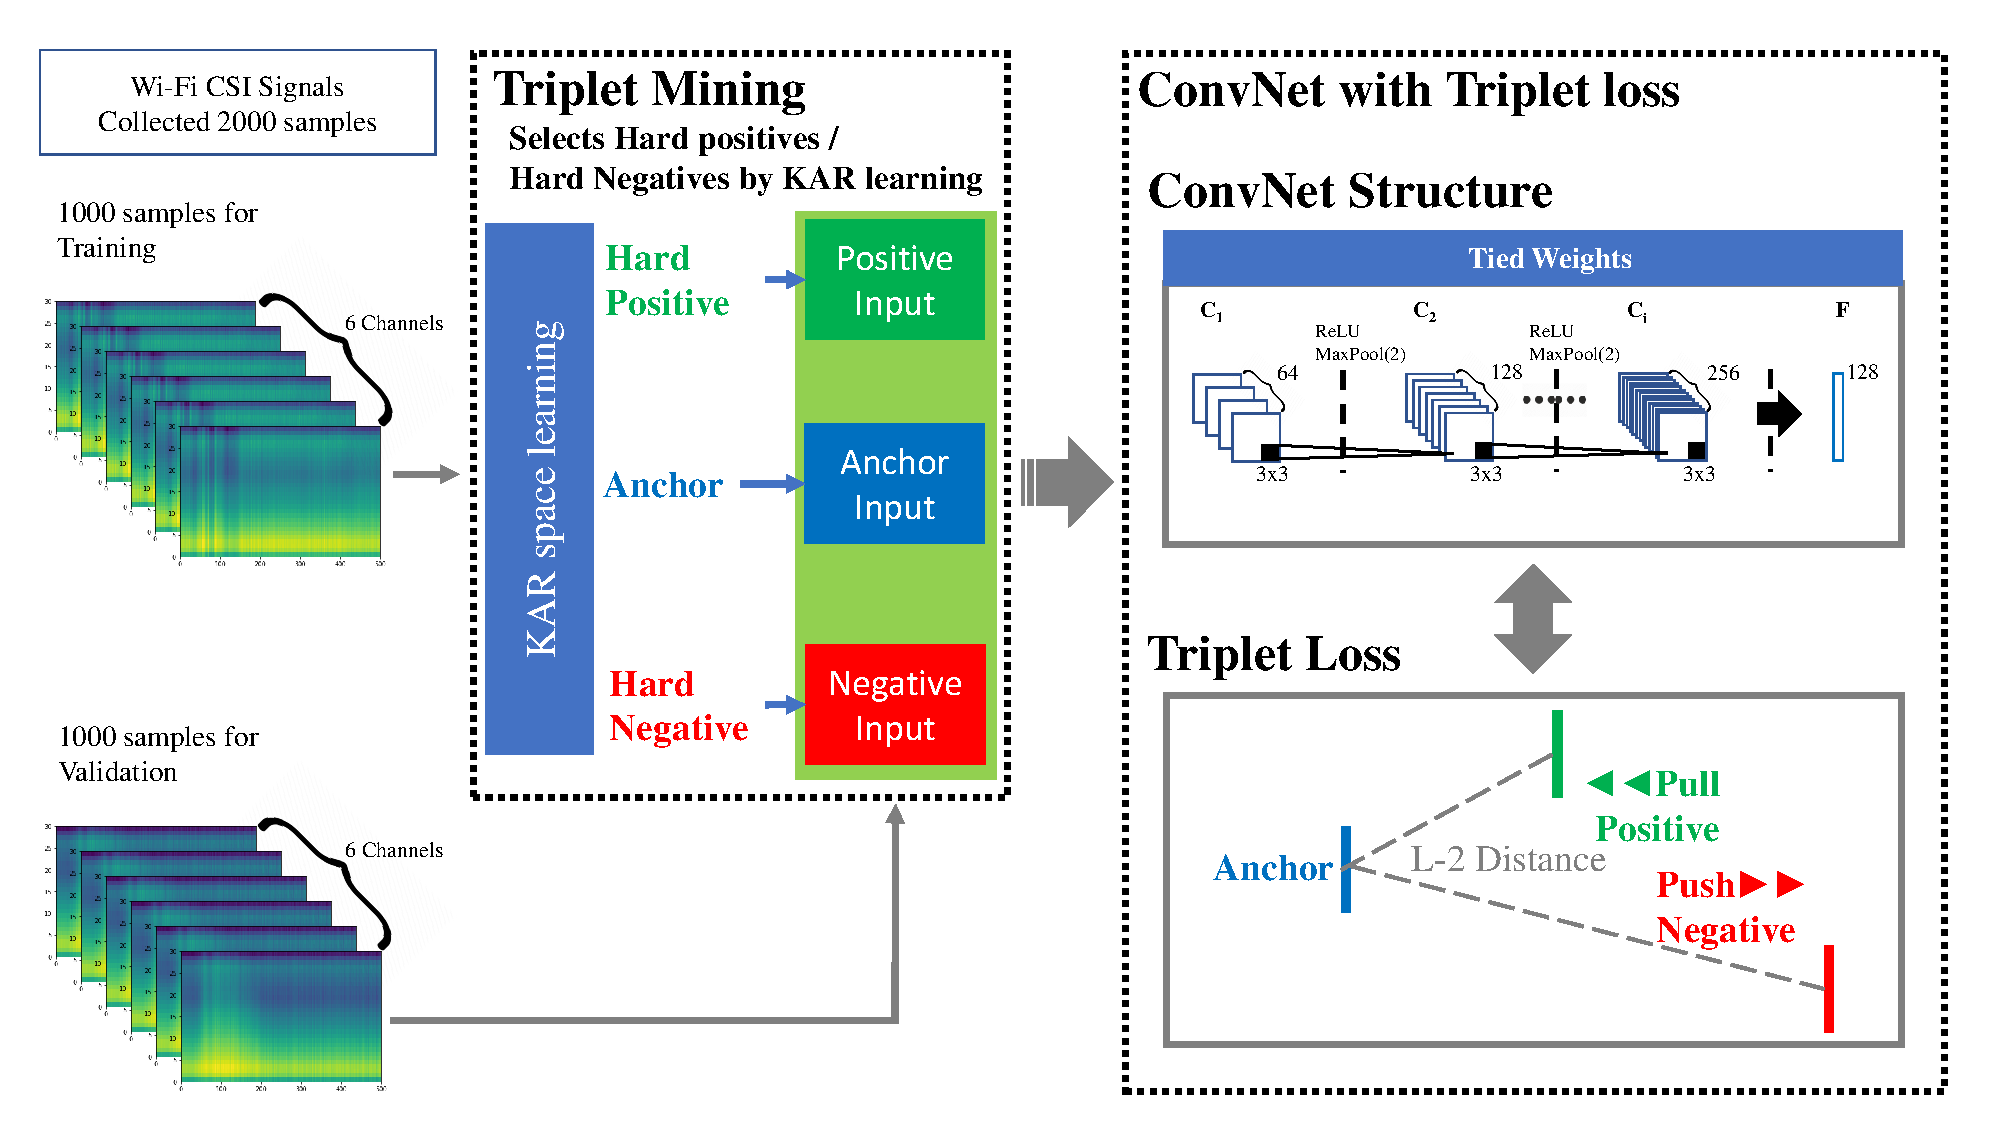
\includegraphics[width=\textwidth]{fig1_tcnn_kar_v1}
    \caption{Structure of the network} \label{fig1}
\end{figure}

% Methods: Triplet loss
\subsection{Triplet loss}

Triplet loss is used to train ConvNet to extract feature vector better from triplet input.
For the $i_{th}$ anchor input signal $\mathbf{X}_{anc,i}$, triplet input is generated by grouping positive input signal $\mathbf{X}_{pos,i}$, which drawn from the same identity for anchor and negative input signal $\mathbf{X}_{neg,i}$, chosen from another identity for the anchor.
Generated triplet input $\left\{\mathbf{X}_{anc,i},\mathbf{X}_{pos,i},\mathbf{X}_{neg,i}\right\}$ is fed into the ConvNet structure one by one and makes anchor, positive and negative feature vectors.

Let $\mathbf{v}_{anc,i}\in{\mathrm{R}}^{d\times1}$, $\mathbf{v}_{pos,i}\in{\mathrm{R}}^{d\times1}$ and $\mathbf{v}_{neg,i}\in{\mathrm{R}}^{d\times1}$ be three feature vectors extracted from the ConvNet structure. 

triplet loss is calculated by comparing positive distance(L-2 distance from anchor to positive feature vector)and negative distance(L-2 distance from anchor to negative feature vector).
ConvNet is trained to maximize gap between positive distance to negative distance more than margin $\alpha$.

The triplet loss for the inputs can be calculated as follows:

\begin{equation}
    loss = \sum_i^N max\left({ \left[ {\left\| {{\mathbf{v}_{anc,i}} - {\mathbf{v}_{pos,i}}} \right\|_2^2} - {\left\| {{\mathbf{v}_{anc,i}} - {\mathbf{v}_{neg,i}}} \right\|_2^2}  + \alpha \right]}, 0 \right)
\end{equation} 

where N is size of the mini-batch.
note that triplet loss can down to 0 when negative distance is longer than positive distance more than margin $\alpha$.
if we select proper triplet for training, we can avoid this problem and make convergence of the loss function faster. This can be done by selecting hard triplet.

% Methods: KAR learning

\subsection{Triplet mining by the kernel and the range space learning}

% importance of selecting hard pos/neg
Regarding to \cite{schroff2015facenet}, it is important to take hard positive and hard negative sample for faster convergence of the loss when training triplet networks.
hard positive sample means distance between feature vectors from positive signal to anchor signal is the greatest, while hard negative sample means distance between feature vectors from negative signal to anchor signal is the smallest.

% methods of KAR learning
since we don't know which is the hard sample before training the network, we train multilayer feedforward neural network to mine the hard positive and the hard negative from traning dataset.
For training multilayer neural network, we adopted gradient-free the kernel and the range (KAR) space projection learning. \cite{toh2018learning,toh2018gradient}.

% Karnet structure and mining samples.
Let the training dataset $\mathbf{X}\in{\mathrm{R}}^{m \times (n+1)}$ and $\mathbf{G}\in{\mathrm{R}}^{m \times n}$ is network outputs.
Multilayer neural network structure is shown below:

\begin{equation}
    \mathbf{G} = \sigma\left(\left[\mathbf{1},\sigma\left(\dots\left[\mathbf{1},\sigma\left(\left[\mathbf{1},\sigma\left(\mathbf{X}\mathbf{W}_{1}\right)\right]\mathbf{W}_{2}\right)\right]\dots\mathbf{W}_{(i-1)}\right)\right]\mathbf{W}_{i}\right),
\end{equation}

$\mathbf{W}_{1}\in{\mathrm{R}}^{(n+1) \times h_{1}}$,$\mathbf{W}_{2}\in{\mathrm{R}}^{(h_{1}+1) \times h_{2}}$,$\dots,\mathbf{W}_{i}\in{\mathrm{R}}^{(h_{(i-1)}+1) \times n}$,$\mathbf{1}=\left[1,\dots,1\right]^{T}\\
\in{\mathrm{R}}^{m \times 1}$ and $\sigma(.)$ is activation function.

when all weights have been learned, for given anker signal, hard negative samples can be mined among the distance of network output of desired signal $\mathbf{G}$ is below the threshold.

% training KARnet
Network learning is archived using one-hot encoded target $\mathbf{Y}\in{\mathrm{R}}^{m \times n}$ instead of network output $\mathbf{G}$.
After that, we have the weight matrix $\mathbf{W}_{1}\dots\mathbf{W}_{i}$ to train. the weight matrix can be separated into weights and bias term as
$\mathbf{W}_{2}\dots\mathbf{W}_{i}$ = 
$\begin{bmatrix}
\mathbf{w}_{2}^{T}\\\mathnormal{W}_{2}
\end{bmatrix}
\dots
\begin{bmatrix}
\mathbf{w}_{i}^{T}\\\mathnormal{W}_{i}
\end{bmatrix}$.

after assign random weights to $\mathbf{W}_{1}\dots\mathbf{W}_{i}$ , we get $\mathbf{W}_{1}$. it is solved as follows:

\begin{equation}
    \left[\sigma^{-1}\left(\mathbf{Y}\right)-\mathbf{1}\cdot\mathbf{w}_{i}^{T}\right]\mathnormal{W}_{i}^\dagger = 
    \sigma\left(\dots\left[\mathbf{1},\sigma\left(\left[\mathbf{1},\sigma\left(\mathbf{X}\mathbf{W}_{1}\right)\right]\mathbf{W}_{2}\right)\right]\dots\mathbf{W}_{(i-1)}\right)
\end{equation}

%\begin{multline*}
\begin{equation}
    \begin{aligned}
        \Rightarrow
        \biggl[\sigma^{-1}\biggl(
        \dots
        \biggl[\sigma^{-1}\biggl(
            \left[\sigma^{-1}\left(\mathbf{Y}\right)-\mathbf{1}\cdot\mathbf{w}_{i}^{T}\right]\mathnormal{W}_{i}^\dagger
        \biggr)
        - \mathbf{1}\cdot\mathbf{w}_{(i-1)}^{T}\biggr]\mathnormal{W}_{(i-1)}^{\dagger}
        \dots\biggr)\\
        - \mathbf{1}\cdot\mathbf{w}_{2}^{T}\biggr]\mathnormal{W}_{2}^{\dagger} 
        = \sigma\left(\mathbf{X}\mathbf{W}_{1}\right)
    \end{aligned}
\end{equation}
%\end{multline*}

%\begin{multline*}
\begin{equation}
    \begin{aligned}
        \Rightarrow
        \mathbf{X}^{\dagger}\sigma^{-1}\biggl(
        \biggl[\sigma^{-1}\biggl(
        \dots
        \biggl[\sigma^{-1}\biggl(
            \left[\sigma^{-1}\left(\mathbf{Y}\right)-\mathbf{1}\cdot\mathbf{w}_{i}^{T}\right]\mathnormal{W}_{i}^\dagger
        \biggr)
        - \mathbf{1}\cdot\mathbf{w}_{(i-1)}^{T}\biggr]\mathnormal{W}_{(i-1)}^{\dagger}
        \dots\biggr)\\
        - \mathbf{1}\cdot\mathbf{w}_{2}^{T}\biggr]\mathnormal{W}_{2}^{\dagger}
        = \mathbf{W}_{1}
    \end{aligned}
\end{equation}
%\end{multline*}

after getting $\mathbf{W}_{1}$, $\mathbf{W}_{2}$ can also be optimized

%\begin{multline*}
\begin{equation}
    \begin{aligned}
        \Rightarrow
        \left(\sigma\left(\mathbf{X}\mathbf{W}_{1}\right)\right)^{\dagger}
        \biggl(\dots
        \biggl[\sigma^{-1}\biggl(
            \left[\sigma^{-1}\left(\mathbf{Y}\right)-\mathbf{1}\cdot\mathbf{w}_{i}^{T}\right]\mathnormal{W}_{i}^\dagger
        \biggr)
        - \mathbf{1}\cdot\mathbf{w}_{(i-1)}^{T}\biggr]\mathnormal{W}_{(i-1)}^{\dagger}
        \dots\biggr)\\
        = \mathbf{W}_{2}
    \end{aligned}
\end{equation}
%\end{multline*}

Repeat this process recursively until all weight maxtrix values are obtained.
finally, $\mathbf{W}_{i}$ can be obtained as follows:

\begin{equation}
    \mathbf{W}_{i} = \left[\mathbf{1},\sigma\left(\dots\left[\mathbf{1},\sigma\left(\left[\mathbf{1},\sigma\left(\mathbf{X}\mathbf{W}_{1}\right)\right]\mathbf{W}_{2}\right)\right]\dots\mathbf{W}_{(i-1)}\right)\right]^{\dagger}\sigma^{-1}\left(\mathbf{Y}\right),
\end{equation}


% Methods: ConvNets
\subsection{ConvNet Structures}

To design the proposed networks, we firstly need to select the feature extracting networks which convert the triplet data into a feature vector. In this work, we utilize the ConvNet structure \cite{lecun1998gradient} as a feature extractor since the three-dimensional data format of our preprocessed input signal can be regarded as an image data format with multiple channels. 

Our ConvNet structure (See Fig~\ref{fig1} (b)) for the network consists of $i$ convolutional layers $\mathbf{C}_{i}$ and one fully-connected layer $\mathbf{F}$. The number of convolutional filters to be trained in each layer is empirically chosen as $\{64, 128, ...,  2^{6+i}\}$, with fixed filter size of $3\times3$ and stride of 1. The Rectified Linear (ReLU) function as an activation function and the max-pooling layers are applied between each convolutional layers. The features from the last convolutional layer are directly flattened into a single vector.
we used sigmoid activation at ConvNet output and L-2 normalize output vectors to prevent negative distance when calculating triplet loss.

%Since the networks utilize three ConvNet structures which ties the weights each other, noting here that three structures described in Fig~\ref{fig1} (b) are actually the same model.

\section{Experiments}

% Dataset
\subsubsection{Dataset}
 To evaluate validation performance of proposed system, Wi-Fi CSI signature dataset from \cite{moon2017air} was used.
 % pre-processing
 Since every Wi-Fi signature signal has different data size, we firstly adopted the gradient operation with respect to the time instance to measure the short time energy. Data points with the highest short-time energy within the time period are then manually selected as the starting and the ending points of the in-air signature action.
 
 Subsequently, the Fast Fourier Transform based re-sampling method \cite{moon2017air} is implemented to unify the length of the signals. As a result, three-dimensional Wi-Fi signature signals with unified data size are obtained as the input of the ConvNet structure in the network.
 % description
 we utilized 2000 Wi-Fi CSI signature signals (4 directions $\times$ 50 identities $\times$ 10 samples) which is dimension of (500 packets $\times$ 30 subcarriers $\times$ 6 antennas). 
 

% Network Learning
\subsubsection{ConvNet structure}
 We impose a triplet loss objective on our classifier.
This objective is combined with standard backpropagation algorithm.
 We initialized all network weights in the convolutional layers from a normal distribution with zero-mean and a standard deviation of 0.01. Biases were also initialized from a normal distribution, but with mean 0.5 and standard deviation 0.01.
 all layers are L-2 regularized using parameters of 0.0002. for output layer, regularization is 0.001

 For KARnet trainied multilayer neural networks, we set 2 layer and number of neurons are [1024,128]. initialized as uniform distribution over [0, 1).
 activation and inverse activation functions are [arctan, tan].

\subsubsection{Results}
\subsubsection{Training Efficiency}

\section{Conclusion}

%
% ---- Bibliography ----
%
% BibTeX users should specify bibliography style 'splncs04'.
% References will then be sorted and formatted in the correct style.
%
%\bibliographystyle{splncs04}
%\bibliography{mybibliography}
%


%\begin{thebibliography}{8}

\bibliographystyle{splncs04}
\bibliography{bib_acpr}

%\end{thebibliography}

\end{document}